% !TeX root = ../main.tex

% Edit this title for each week's entry.
\section{Week 4: Mitigating Violated Assumptions}

\subsection{Review: Assumptions and Residual Plots}

\begin{remark}[The 4 Assumptions (Week 3)]
    Assumptions are about the \textbf{population}, not the sample, and are
    made implicitly \textbf{every} time we fit a model. All four are packed into
    \[\boldsymbol\epsilon\mid\mathbf{X}\sim N_n(\underbrace{\mathbf{0}}_{\text{linearity}},\ \underbrace{\sigma^2}_{\text{const.\ var.}}\underbrace{\mathbf{I}}_{\text{uncorr.}})
    \quad\text{or}\quad \mathbf{Y}\mid\mathbf{X}\sim N_n(\mathbf{X}\boldsymbol\beta,\sigma^2\mathbf{I}),\]
    with the $N$ itself being the normality assumption.
    \begin{enumerate}
        \item \textbf{Linearity} (mean zero errors): $E(\boldsymbol\epsilon\mid\mathbf{X})=\mathbf{0}$, i.e.\ $E(\mathbf{Y}\mid\mathbf{X})=\mathbf{X}\boldsymbol\beta$
        \item \textbf{Uncorrelated errors}: $\Cov(\epsilon_i,\epsilon_j)=\Cov(y_i,y_j)=0$
        \item \textbf{Constant variance}: $\Var(\boldsymbol\epsilon\mid\mathbf{X})=\Var(\mathbf{Y}\mid\mathbf{X})=\sigma^2\mathbf{I}$
        \item \textbf{Normal errors}: $\epsilon_i\overset{iid}\sim N(0,\sigma^2)$
    \end{enumerate}
    \aside{1--3 are needed for OLS. Normality is not needed for OLS, but is
    needed for inference.}
\end{remark}

\heading{Spotting Violations with Residuals}
\begin{itemize}
    \item \rb{Linearity}: any systematic pattern, especially curves or other functions of predictors.
    \item \rb{Uncorrelated errors}: large clusters of many points, or a pattern in \textbf{time}
    or other sequencing information. \aside{Check how the data was collected.}
    \item \rb{Constant variance}: any systematic pattern, especially a fanning/funnel pattern
    with increasing or decreasing spread.
    \item \rb{Normality}: QQ plot --- look for stark deviations/curving/wiggling from the
    diagonal line \aside{(minimal deviations ok)}.
\end{itemize}

\subsection{Introduction to Transformations}

\begin{definition}[Transformed Model]
    The main reasons to transform are to overcome \textbf{non-linearity} and
    \textbf{non-constant variance}. We fit
    \[g_Y(Y)=\beta_0+\beta_1g_{X_1}(X_1)+\beta_2g_{X_2}(X_2)+\cdots+\epsilon\]
    where the $g(\cdot)$ are transformations applied to the original data.
    \begin{itemize}
        \item We can transform any subset of the response and predictors.
        \item We can only interpret the model in terms of the
        \emph{transformed} predictors/response.
    \end{itemize}
\end{definition}

\heading{Choosing a Transformation}
\begin{enumerate}
    \item Plot the response vs.\ the predictors (or residuals) to look for an appropriate transformation.
    \item Choose a transformation to try to fix the residual plot.
    \item Plot again to see if the issue was fixed.
\end{enumerate}
\textbf{Drawback}: may make interpretation of the estimated coefficients difficult.
\textbf{Advantage}: often improves prediction and inference.

\begin{definition}[Common Transformations]
    \begin{itemize}
        \item \textbf{Logarithmic}: $g(z)=\log(z)$ \aside{(usually natural log;
        make sure the variable is strictly positive)}
        \item \textbf{Power}: $g(z)=z^\lambda$ for $\lambda>0$
        \item \textbf{Inverse power}: $g(z)=1/z^\lambda$ for $\lambda>0$
    \end{itemize}
    \aside{$\lambda$ is usually a ``nice'' number.} These can be applied to
    predictors or the response; e.g.\ from SLR $Y=\beta_0+\beta_1X+\epsilon$:
    \[Y=\beta_0+\beta_1X^2+\epsilon,\qquad \log(Y)=\beta_0+\beta_1X+\epsilon,\qquad \sqrt Y=\beta_0+\beta_1\exp(X)+\epsilon\]
    \aside{The last two are no longer linear in $Y$.}
\end{definition}

\begin{remark}[Transformations for Skewed Data]
    Instead of $X$ use $X^*=f(X)$ (same for $Y$); any numerical variable can be transformed.
    \begin{itemize}
        \item \textbf{Right skew}: $\log(x-c)$, $\sqrt{x-c}$, etc.
        \item \textbf{Left skew}: $x^2$, $\sqrt{c-x}$, $\log(c-x)$, etc.
        \item Check graphically whether it improved.
    \end{itemize}
    There are analytic methods to help choose a transformation (Box--Cox, below);
    these common ones are often the recommended options.
\end{remark}

\subsection{Variance Stabilizing Transformations}

\begin{definition}[Variance Stabilizing Transformation (VST)]
    A transformation that specifically targets violation of
    \textbf{constant variance}. It is applied to the \textbf{response $Y$ only}
    \aside{--- because in $Y=X\beta+\epsilon$, the variation is in $\epsilon$; there
    is no randomness associated with $X$.} Best practice: select transformations
    that target the violation you observe.
\end{definition}

The choice depends on the exact situation and data:
\begin{itemize}
    \item Identifiable data type (e.g.\ count data, binary data) or specific variable context
    \item Experience from similar contexts or data types
    \item No one transformation works for every model --- trial and error
\end{itemize}

\begin{center}
    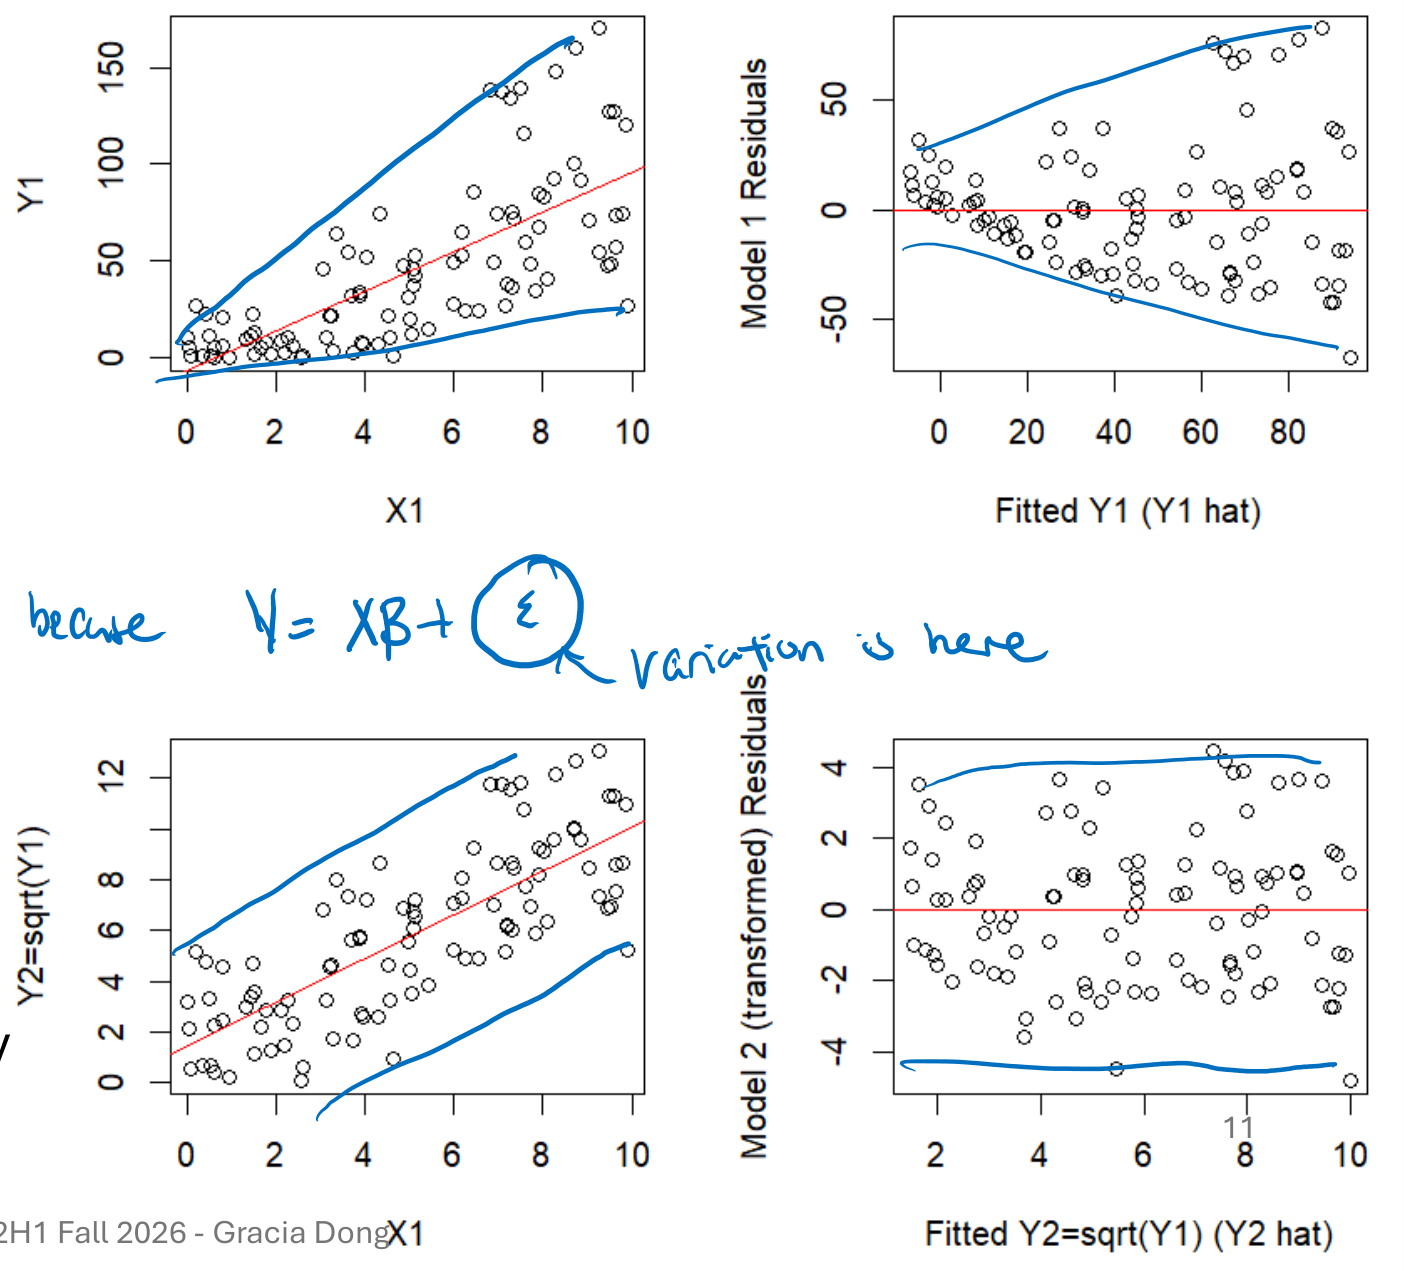
\includegraphics[width=0.6\linewidth]{figures/w4_vst_sqrt.png}
    \\[2pt] \textit{\small Top: $Y_1$ vs.\ $X_1$ and residuals fan out. Bottom: after
    $Y_2=\sqrt{Y_1}$, the residual band is roughly constant.}
\end{center}

\begin{proposition}[Delta Method Approximation]
    Let $f(Y)$ be the transformation. First-order Taylor expansion around the mean:
    \[f(Y)=f\big(E(Y)\big)+f'\big(E(Y)\big)\big(Y-E(Y)\big)+\cdots\]
    Take variance of both sides. $f(E(Y))$, $f'(E(Y))$ and $E(Y)$ are
    \emph{constants}, so $\Var(f(E(Y)))=0$ and the covariance term is
    $\Cov(\text{constant},\text{random})=0$, leaving
    \[\boxed{\Var\big(f(Y)\big)\approx\big[f'\big(E(Y)\big)\big]^2\Var(Y)}\]
    The correct choice of $f$ cancels out the non-constant part of $\Var(Y)$.
\end{proposition}

\begin{example}[Poisson Response]
    Suppose $Y\mid X\sim\text{Poi}(X)$, so $E(Y\mid X)=\Var(Y\mid X)=X$.
    \aside{This also violates normality, but focus on non-constant variance for now.}
    Is $f(Y)=\sqrt Y$ variance-stabilizing?
    \\\db{$f(y)=y^{1/2}\Rightarrow f'(y)=\tfrac12y^{-1/2}$, so $f'(E(Y\mid X))=\tfrac12X^{-1/2}$. Then
    \[\Var\big(f(Y)\mid X\big)\approx\Big(\tfrac12X^{-1/2}\Big)^2X=\tfrac14,\]
    which is \dbb{constant}.}
    \begin{center}
        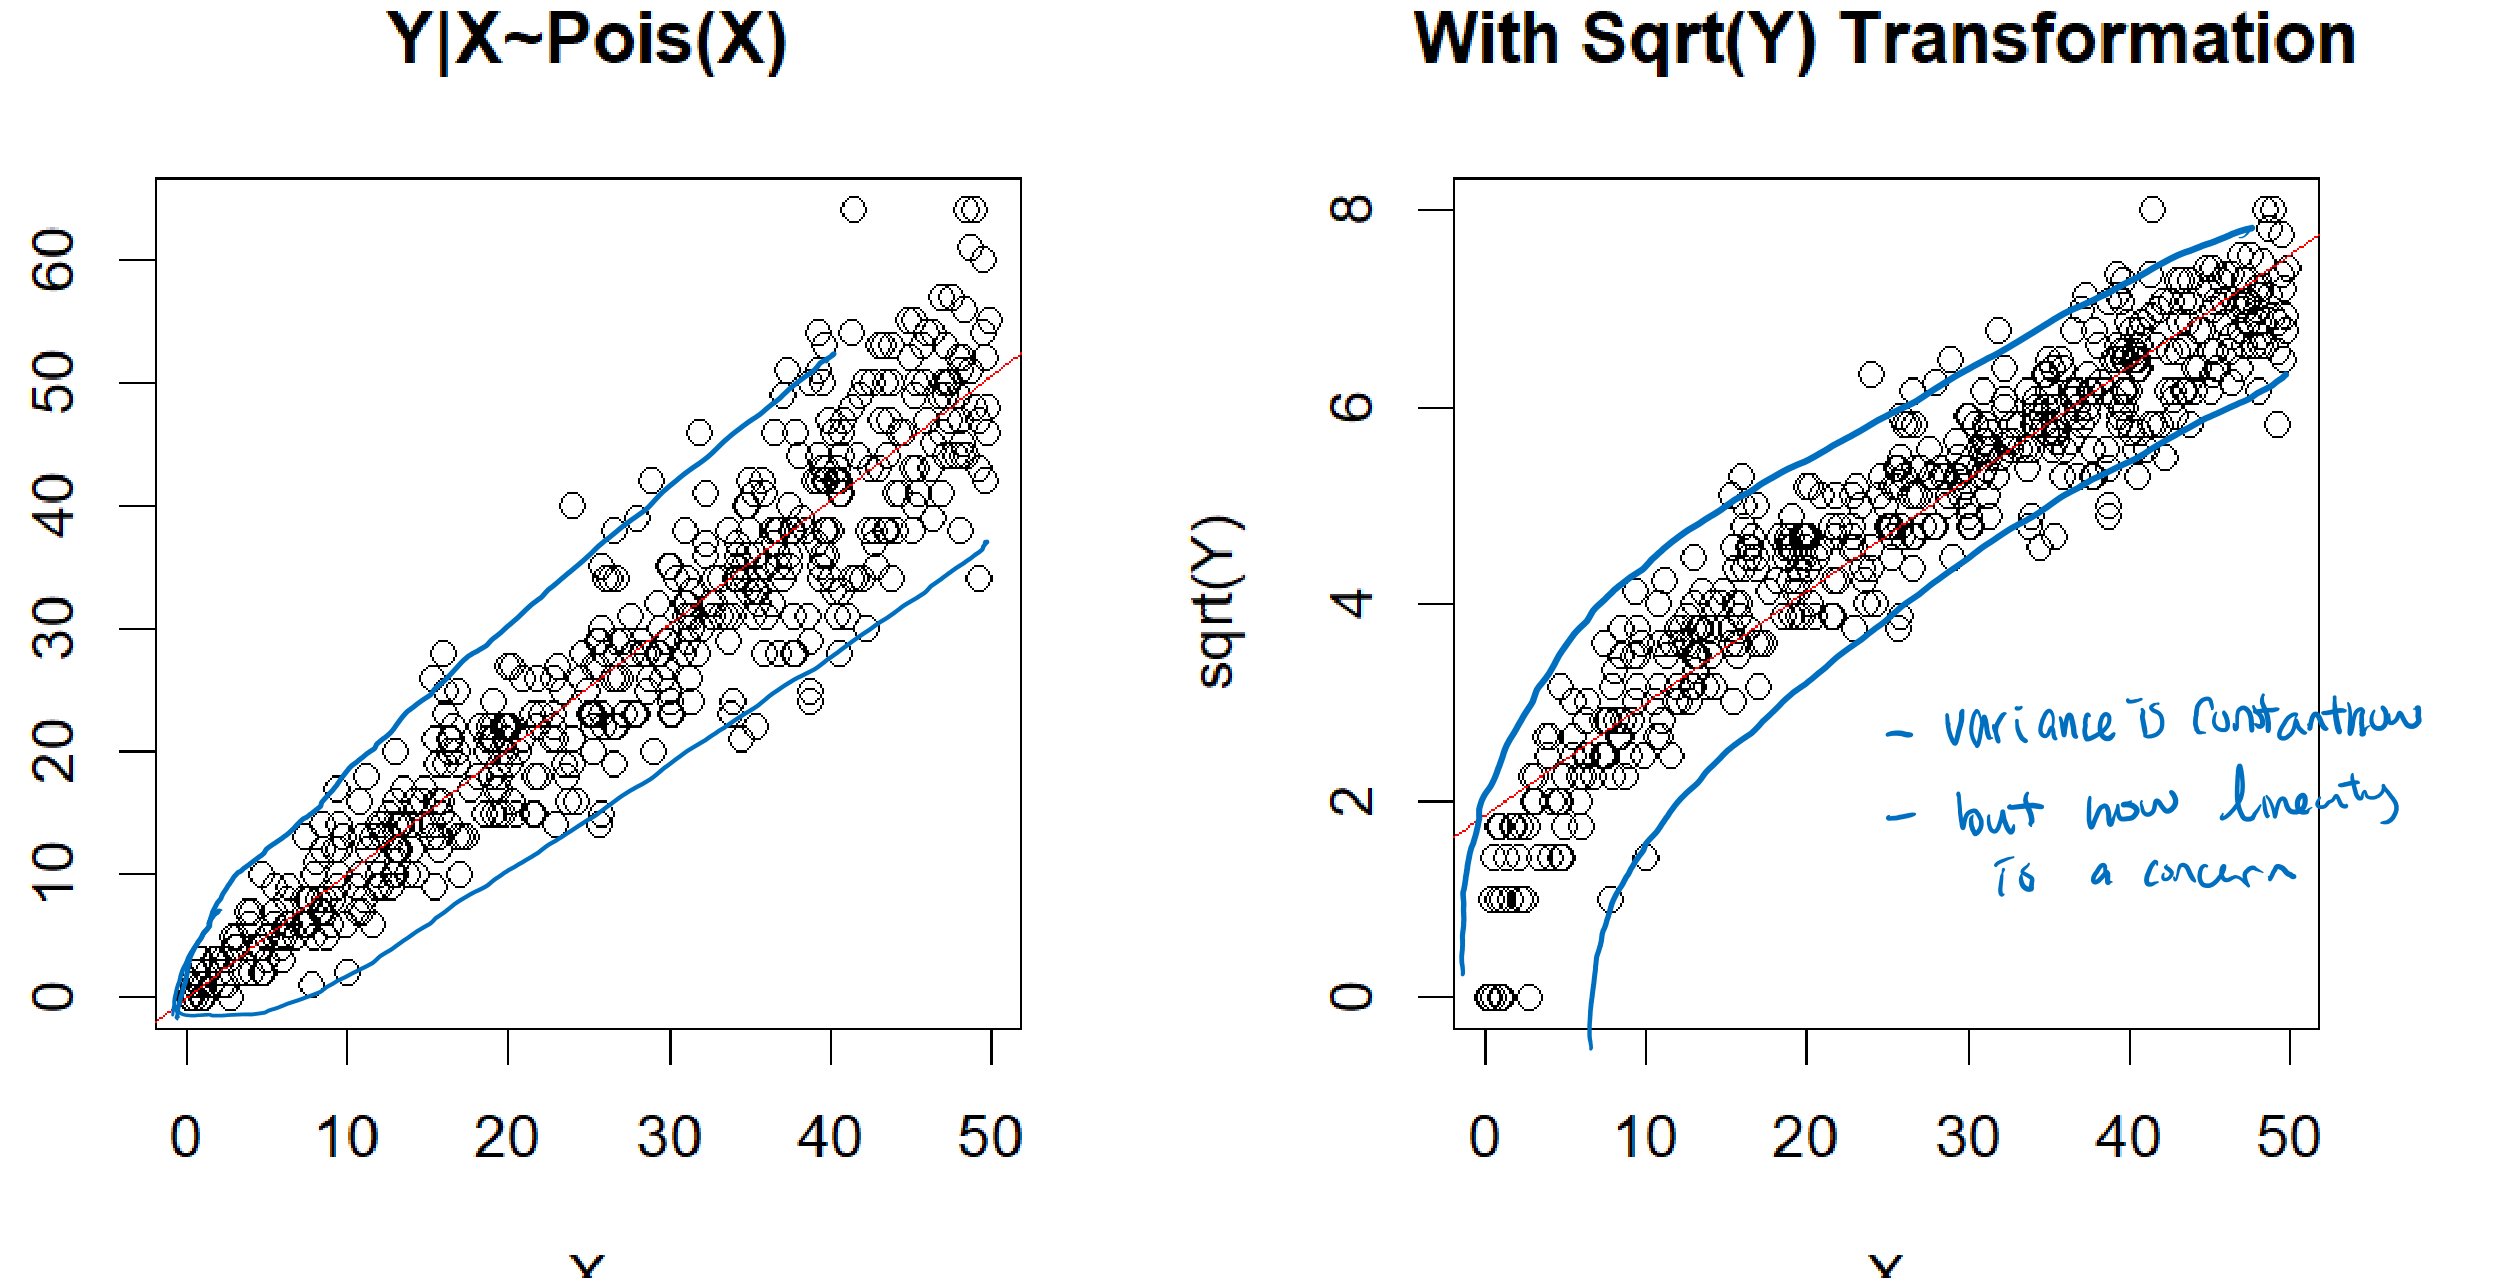
\includegraphics[width=0.62\linewidth]{figures/w4_poisson_sqrt.png}
    \end{center}
    \aside{After $\sqrt Y$ the variance is constant, but now linearity is a concern.}
\end{example}

\heading{Notes on VSTs}
\begin{itemize}
    \item Only transform $Y$.
    \item Can potentially make other assumption violations worse.
    \item Pick based on what the plots look like and the direction of the funnel:
    \begin{itemize}
        \item No obvious choice; common ones when variance increases with $Y$: $\ln(y-c)$, $\sqrt{y-c}$, etc.
        \item If variance decreases with $Y$, flip to $\ln(c-y)$, \dots
    \end{itemize}
    \item Apply transformation, fit model, then plot again.
\end{itemize}

\begin{proposition}[Common VSTs]
    \begin{center}
        \begin{tabular}{ll}
            \toprule
            If $\Var(Y\mid X)\propto$ & use $f(Y)\propto$ \\
            \midrule
            $E(Y\mid X)$ & $\sqrt Y$ \aside{(could be $\sqrt{Y-c}$, $\sqrt{c-Y}$, \dots)} \\
            $E(Y\mid X)^2$ & $\log(Y)$ \\
            $E(Y\mid X)^3$ & $1/\sqrt Y$ \\
            $E(Y\mid X)^4$ & $1/Y$ \\
            \bottomrule
        \end{tabular}
    \end{center}
    It can be hard to tell visually what $\Var(Y\mid X)$ is proportional to ---
    try different transformations and check for improvement.
\end{proposition}

\begin{exercise}[Verify the Table]
    Verify each row using $\Var(f(Y)\mid X)\approx[f'(E(Y\mid X))]^2\Var(Y\mid X)$.
    \\\db{Write $\mu=E(Y\mid X)$ and $\Var(Y\mid X)=k\mu^m$.
    $\log$: $f'=1/\mu$, so $\mu^{-2}\cdot k\mu^2=k$.
    $1/\sqrt Y$: $f'=-\tfrac12\mu^{-3/2}$, so $\tfrac14\mu^{-3}\cdot k\mu^3=k/4$.
    $1/Y$: $f'=-\mu^{-2}$, so $\mu^{-4}\cdot k\mu^4=k$.
    All constant.}
\end{exercise}

\subsection{Box--Cox Transformations for Normality}

\begin{remark}[Motivation]
    Last week we eyeballed transformations for linearity from residual plots and
    scatterplots. Whatever ``signal'' the line of best fit misses is most likely a
    missing predictor (e.g.\ an arch in residuals vs.\ Distance $\Rightarrow$ add
    Distance$^2$; a concave $\sqrt Y$ vs.\ $X$ $\Rightarrow$ try $\sqrt X$).
    Sometimes the needed transformation isn't obvious even from residual vs.\
    predictor plots, so we find the ``best'' one \textbf{analytically}.
\end{remark}

\begin{definition}[Box--Cox Transformation (Box \& Cox, 1964)]
    Power transformations, chosen to improve \textbf{normality} violations.
    Can be used on the response, on the predictor(s), or on both simultaneously.
    \aside{Side effect: can help with linearity.} In this class we won't use it
    exactly as intended due to its complexity.
    \\ Further reading: Weisberg \S8.1.2--8.1.3 (pg 188); derivation: Appendix A.12 (pg 312).
\end{definition}

\begin{remark}[Maximum Likelihood]
    Box--Cox uses ML to estimate the power; the estimate gives the best
    approximation to normality among all powers. The normal log-likelihood in SLR
    (assumptions holding) is
    \[\log L(\beta_0,\beta_1,\sigma^2\mid Y)=-\frac n2\log(2\pi)-\frac n2\log(\sigma^2)-\frac1{2\sigma^2}\underbrace{\sum(y_i-\beta_0-\beta_1x_i)^2}_{RSS}\]
    \aside{For MLR, just include more $\beta_jx_j$ in the last term.}
\end{remark}

\begin{definition}[How Box--Cox Works]
    Modify the RSS, i.e.\ fit a new model with a different response:
    \[RSS=\sum\big(\Psi_M(Y,\lambda)-\beta_0-\beta_1x_i\big)^2\]
    \[\Psi_M(\mathbf{Y},\lambda)=\text{gm}(\mathbf{Y})^{1-\lambda}\,\Psi_S(y_i,\lambda)=
    \begin{cases}
        \big(e^{\frac1n\sum\log y_i}\big)^{1-\lambda}\,\dfrac{y_i^\lambda-1}{\lambda}, & \lambda\neq0\\[8pt]
        \big(e^{\frac1n\sum\log y_i}\big)^{1-\lambda}\,\log(y_i), & \lambda=0
    \end{cases}\]
    \begin{itemize}
        \item $\text{gm}(\mathbf{Y})=e^{\frac1n\sum\log y_i}$ is the \textbf{geometric mean}
        of $Y$ \aside{(roughly constant if $n$ is large)}.
        \item $\Psi_S(y_i,\lambda)=\frac{y_i^\lambda-1}{\lambda}$ or $\log(y_i)$ is a
        \textbf{s}caled power transformation.
        \item $\Psi_M(\mathbf{Y},\lambda)$ is a \textbf{m}odified power transformation applied to $\mathbf{Y}$.
    \end{itemize}
    This is very complicated, so for interpretability we instead: get the ML
    estimate $\hat\lambda$ (in R), then just use \hlt{$\mathbf{Y}^{\lambda}$ (or $\log\mathbf{Y}$)}.
\end{definition}

\begin{remark}[Box--Cox on $X$, and on $X$ \& $Y$]
    Predictors: $RSS=\sum\big(y_i-\beta_0-\beta_1\Psi_S(X,\lambda)\big)^2$, with
    $\Psi_S(X,\lambda)=\frac{X^\lambda-1}{\lambda}$ ($\lambda\neq0$) or $\log X$ ($\lambda=0$).
    \\ Both simultaneously:
    $RSS=\sum\big(\Psi_M(Y,\lambda_y)-\beta_0-\beta_1\Psi_S(X,\lambda_x)\big)^2$,
    giving ML estimates $(\hat\lambda_y,\hat\lambda_x)$.
    \\ We use the simpler $Y^{\lambda_y}$ and $X^{\lambda_x}$ (or $\log X$, $\log Y$).
    For MLR the process is the same, just more $\lambda$'s to estimate.
\end{remark}

\begin{remark}[Box--Cox Likelihood --- \textbf{not testable}, reference only]
    Issue: $\mathbf{Y}\mid\mathbf{X}\not\sim N(\mathbf{X}\boldsymbol\beta,\sigma^2\mathbf{I})$;
    we need $\Psi_M$ so that $\Psi_M(\mathbf{Y}\mid\mathbf{X})\sim N(\mathbf{X}\boldsymbol\beta,\sigma^2\mathbf{I})$.
    Modify the log-likelihood and add the Jacobian determinant term (multivariate
    transformation method, STA237):
    \[-\frac n2\ln(2\pi)-\frac n2\ln(\sigma^2)-\frac1{2\sigma^2}\sum_{i=1}^n\big(\Psi(y_i)-\beta_0-\beta_1x_i\big)^2+n(\lambda-1)\log\big(\text{gm}(\mathbf{Y})\big)\]
    and maximize over $\lambda$ (in R).
\end{remark}

\heading{Box--Cox in Practice}
\begin{itemize}
    \item The ML process for $\lambda$ has no closed form, so we use R.
    \item The actual Box--Cox transformations are hard to work with, so use
    \textbf{simpler powers}: much easier to \textbf{interpret} and apply, still close
    to normality, and you avoid figuring out what your variable now means.
    \item Pick something simpler than $\hat\lambda$, e.g.\ $\hat\lambda=0.103\Rightarrow$ use $\ln(Y)$ (close to 0):
    \begin{center}
        \begin{tabular}{cl}
            \toprule
            $\lambda$ & transformation \\
            \midrule
            $0.5$ & square root \\
            $0.33$ & cube root \\
            $0.25$ & fourth root \\
            $0$ & log \\
            $-0.5$ & reciprocal square root \\
            $-1$ & reciprocal (inverse) \\
            \bottomrule
        \end{tabular}
    \end{center}
    \item R reports confidence intervals for $\lambda$ --- use them as a range of possibilities.
\end{itemize}

\subsection{Application and Interpretation of Transformed Models}

\begin{example}[Magazine Data]
    \texttt{mag <- read.csv("magazines.csv")}, 204 magazines. Predict
    $Y=$ \texttt{AdRevenue} from $X_1=$ \texttt{AdPages}, $X_2=$ \texttt{SubRevenue},
    $X_3=$ \texttt{NewsRevenue}.
    \begin{center}
        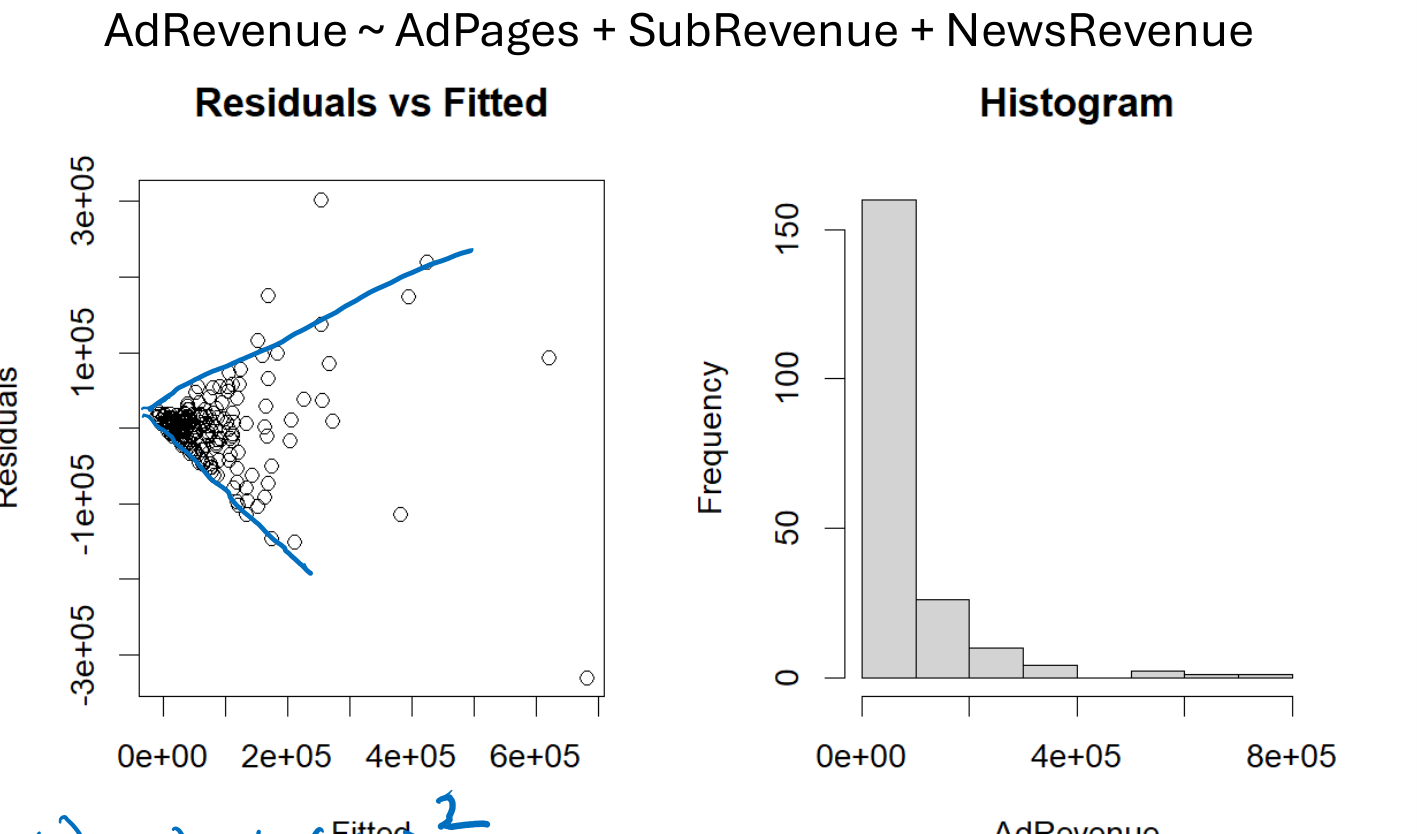
\includegraphics[width=0.55\linewidth]{figures/w4_magazine_resid.png}
    \end{center}
    \db{Issues: residuals fan out ($SD(Y)\propto E(Y)$ visually, so
    $\Var(Y)\propto E(Y)^2$) and \texttt{AdRevenue} is strongly right-skewed
    $\Rightarrow$ \dbb{try a $\log(Y)$ transformation}.}
\end{example}

\begin{example}[Try $\log(\texttt{AdRevenue})$]
    $\log$ and $\sqrt{\ }$ may improve right skew. Some improvement, but other
    violations may be present (the residuals still have a hard left edge).
    \begin{center}
        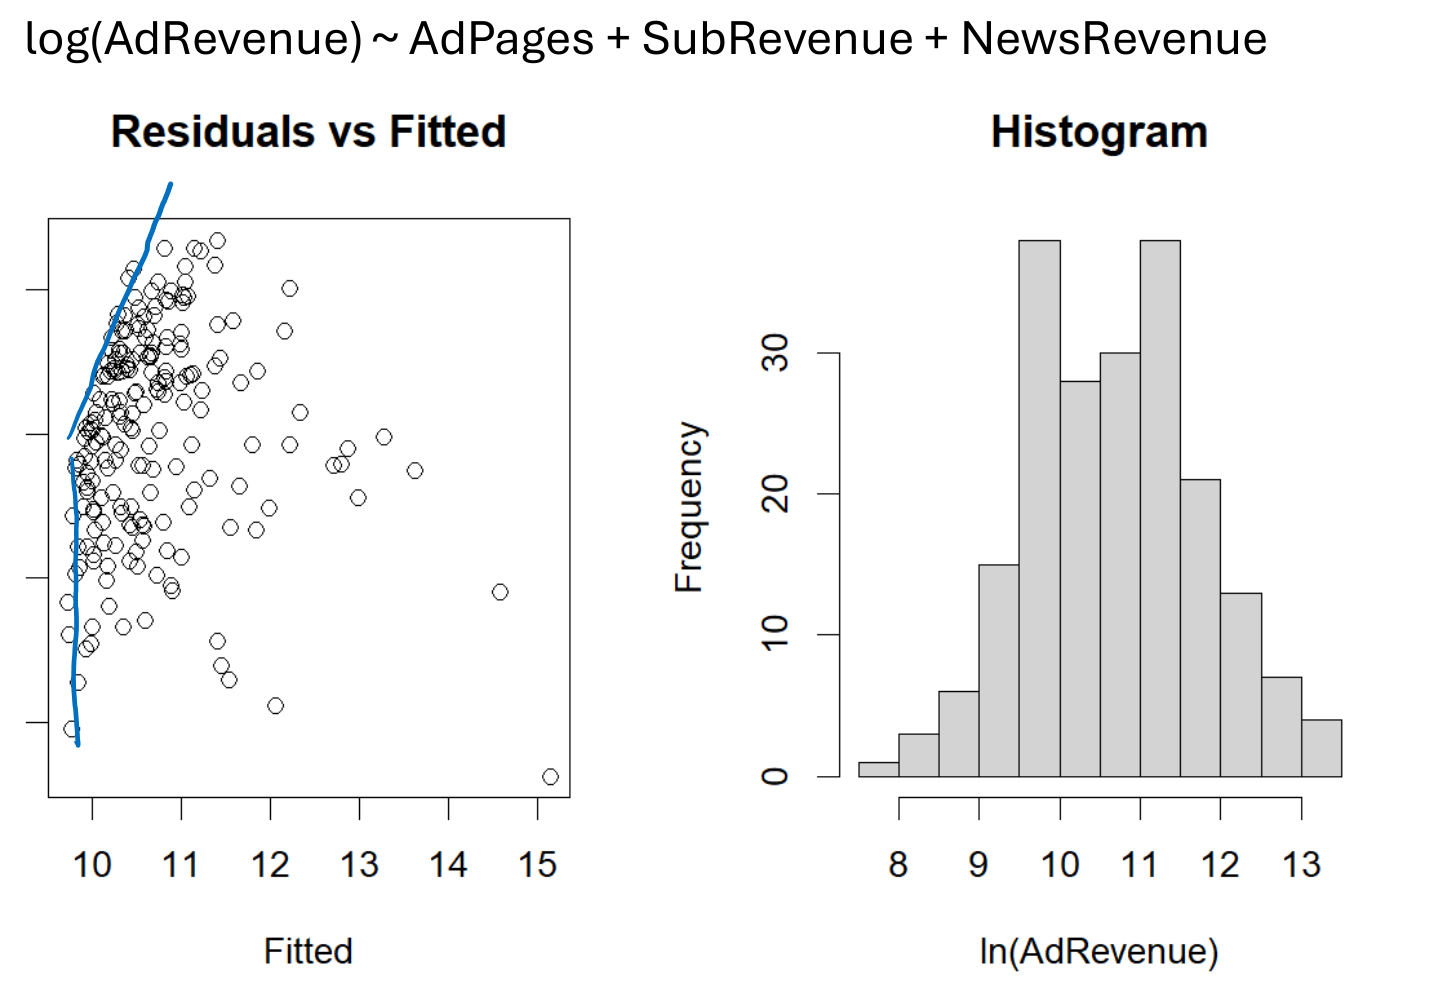
\includegraphics[width=0.55\linewidth]{figures/w4_magazine_log.png}
    \end{center}
    More residual plots for the \emph{original} model show many violations:
    \begin{center}
        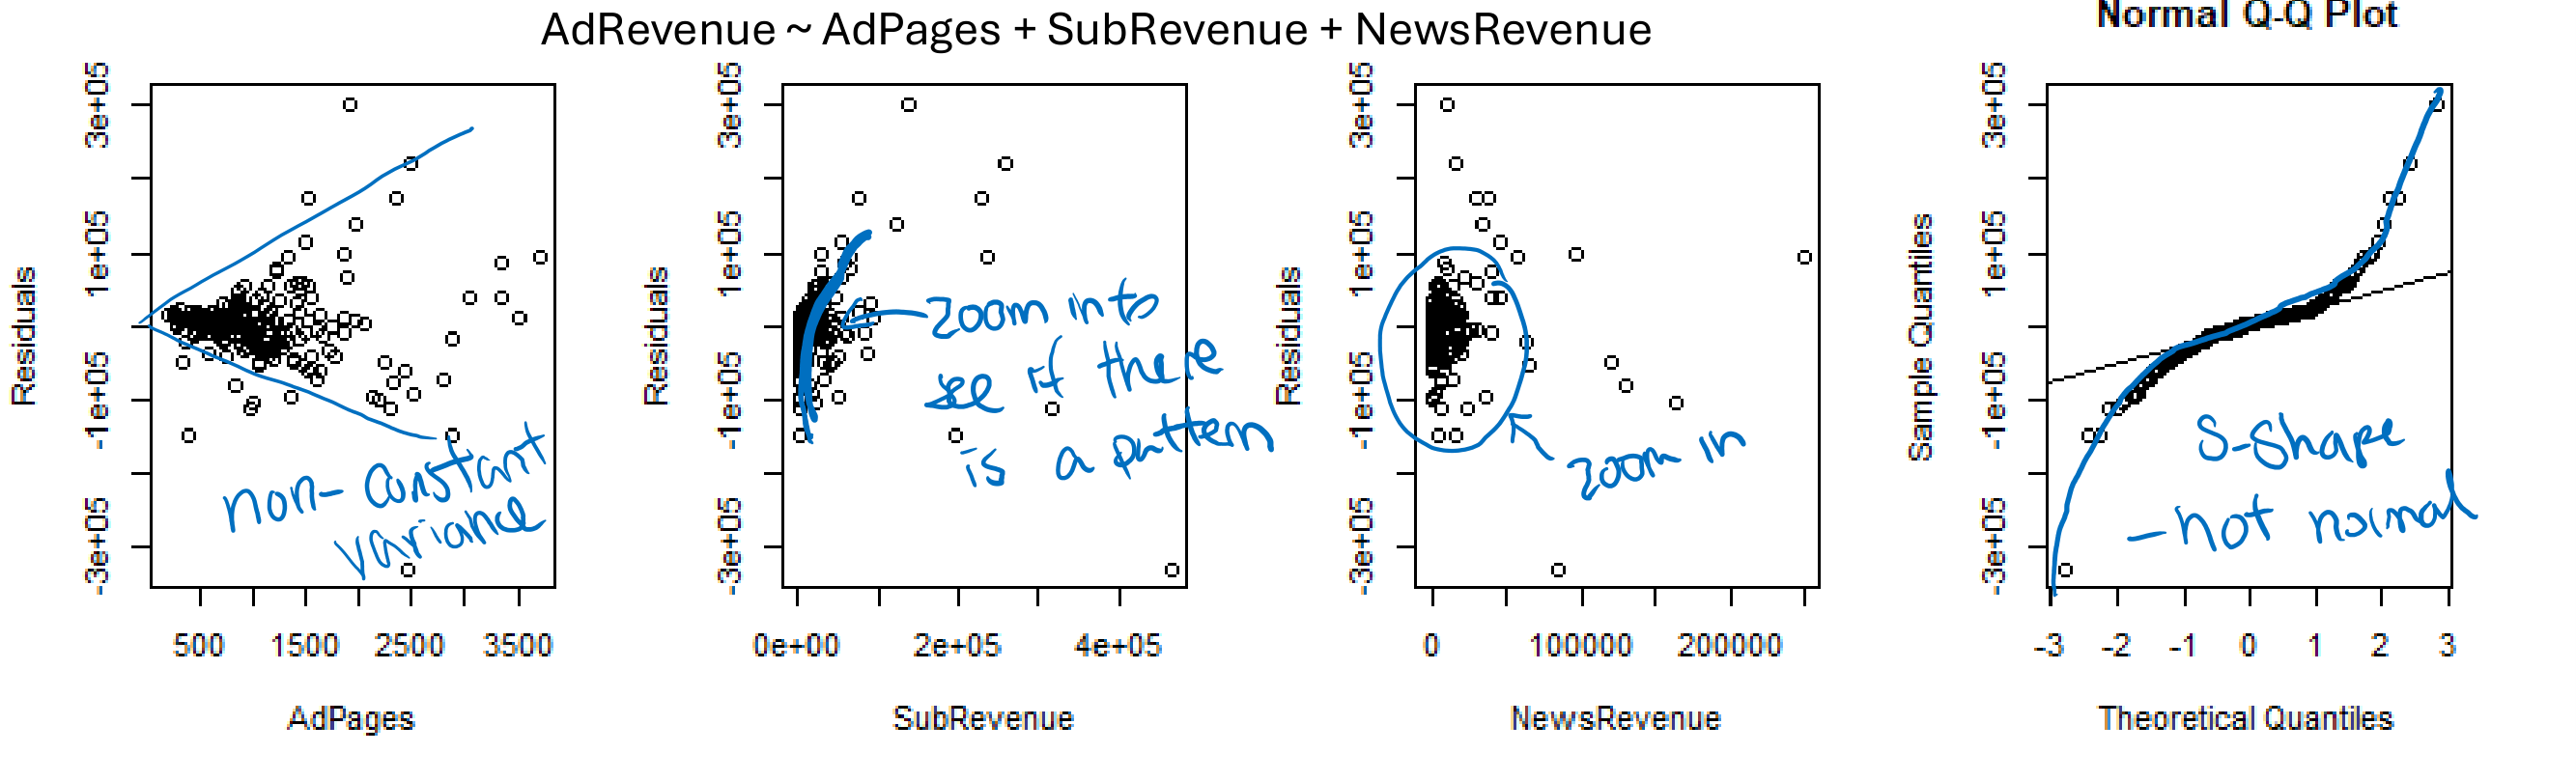
\includegraphics[width=0.95\linewidth]{figures/w4_magazine_allresid.png}
    \end{center}
    \aside{Non-constant variance vs.\ AdPages; zoom in on SubRevenue/NewsRevenue
    clusters to see patterns; S-shaped QQ plot $\Rightarrow$ not normal.}
    So let's try Box--Cox.
\end{example}

\begin{example}[Box--Cox on $Y$]
    Use \texttt{boxCox()} from the \texttt{car} package:
\begin{verbatim}
library(car)     # install.packages("car") for boxCox()
boxCox(model1)   # only transformations on Y; input the whole model
\end{verbatim}
    \begin{center}
        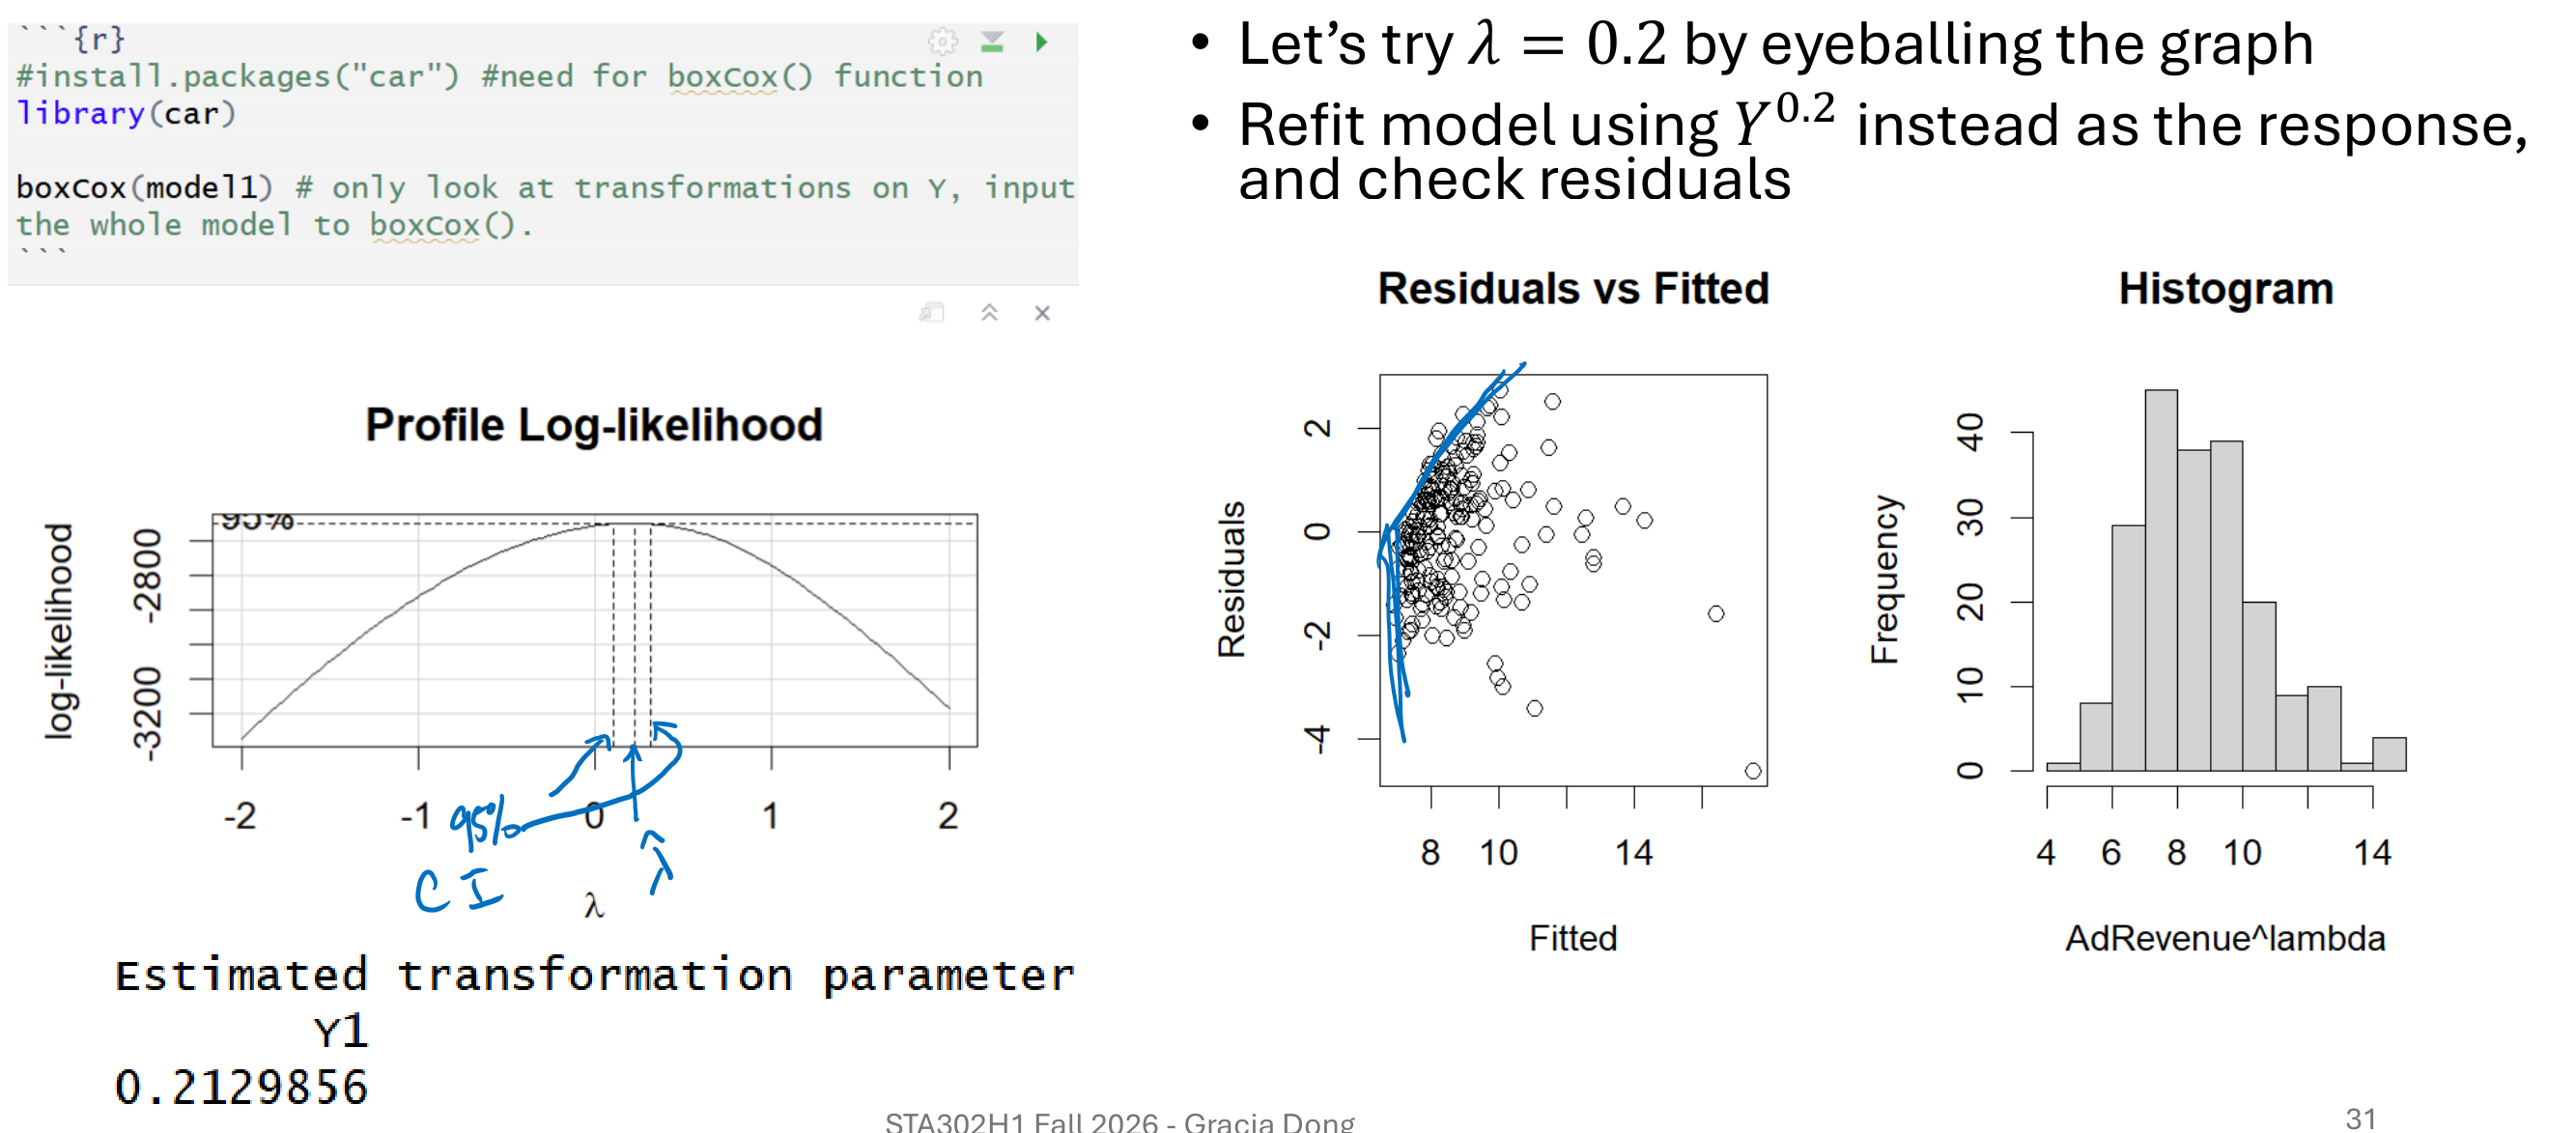
\includegraphics[width=0.9\linewidth]{figures/w4_boxcox_y.png}
    \end{center}
    The profile log-likelihood peaks at $\hat\lambda=0.213$ (dashed lines: $\hat\lambda$
    and its 95\% CI). Eyeballing, try $\lambda=0.2$: refit with $Y^{0.2}$ as the
    response and check residuals. \aside{Histogram is more symmetric, but the
    residuals vs.\ fitted still have an edge.}
\end{example}

\begin{example}[Box--Cox on $X$]
    Use \texttt{powerTransform()} on the predictor columns:
\begin{verbatim}
p <- powerTransform(cbind(mag[,3:5]))  # all columns you may want to transform
summary(p)
\end{verbatim}
    \begin{center}
        \begin{tabular}{lrrrr}
            \toprule
            & Est Power & Rounded Pwr & Wald Lwr & Wald Upr \\
            \midrule
            AdPages & 0.1119 & 0.00 & $-0.0869$ & 0.3107 \\
            SubRevenue & $-0.0084$ & 0.00 & $-0.0973$ & 0.0804 \\
            NewsRevenue & 0.0759 & 0.08 & 0.0106 & 0.1412 \\
            \bottomrule
        \end{tabular}
    \end{center}
    \aside{Ignore the likelihood ratio tests in the output. I would personally round
    0.08 again to 0.} Refit $Y^{0.2}\sim\log(X_1)+\log(X_2)+\log(X_3)$ ($Y^{0.2}$ from the
    previous slide) and check residuals:
    \begin{center}
        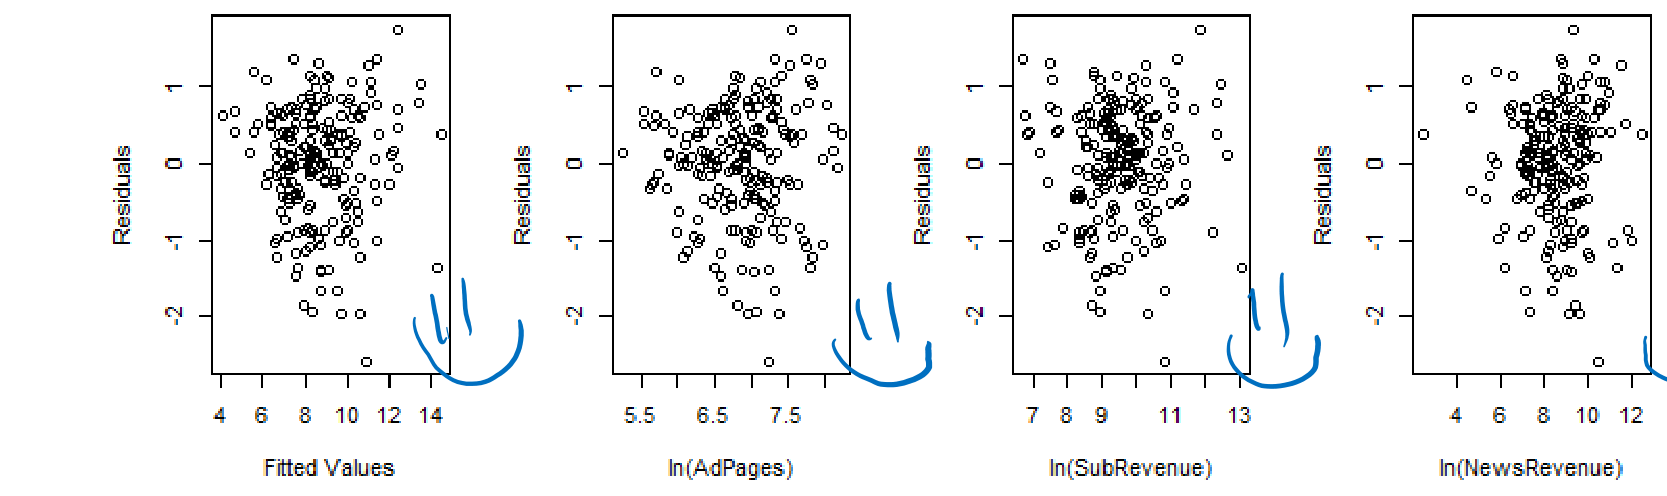
\includegraphics[width=0.85\linewidth]{figures/w4_boxcox_x_resid.png}
    \end{center}
    \aside{Residual plots look fine; mild C shape in QQ plot --- maybe OK, not super concerned.}
\end{example}

\begin{example}[Box--Cox on $X$ and $Y$ Simultaneously]
    Same function, now including the response column:
\begin{verbatim}
p <- powerTransform(cbind(mag[,2:5]))  # include X and Y here
summary(p)
\end{verbatim}
    \begin{center}
        \begin{tabular}{llrrrr}
            \toprule
            && Est Power & Rounded Pwr & Wald Lwr & Wald Upr \\
            \midrule
            $Y$ & AdRevenue & 0.1071 & 0.11 & 0.0299 & 0.1843 \\
            $X_1$ & AdPages & 0.0883 & 0.00 & $-0.0755$ & 0.2521 \\
            $X_2$ & SubRevenue & $-0.0153$ & 0.00 & $-0.0862$ & 0.0557 \\
            $X_3$ & NewsRevenue & 0.0763 & 0.08 & 0.0115 & 0.1410 \\
            \bottomrule
        \end{tabular}
    \end{center}
    \aside{Round 0.11 and 0.08 again to 0.} Refit
    $\log(Y)\sim\log(X_1)+\log(X_2)+\log(X_3)$:
    \begin{center}
        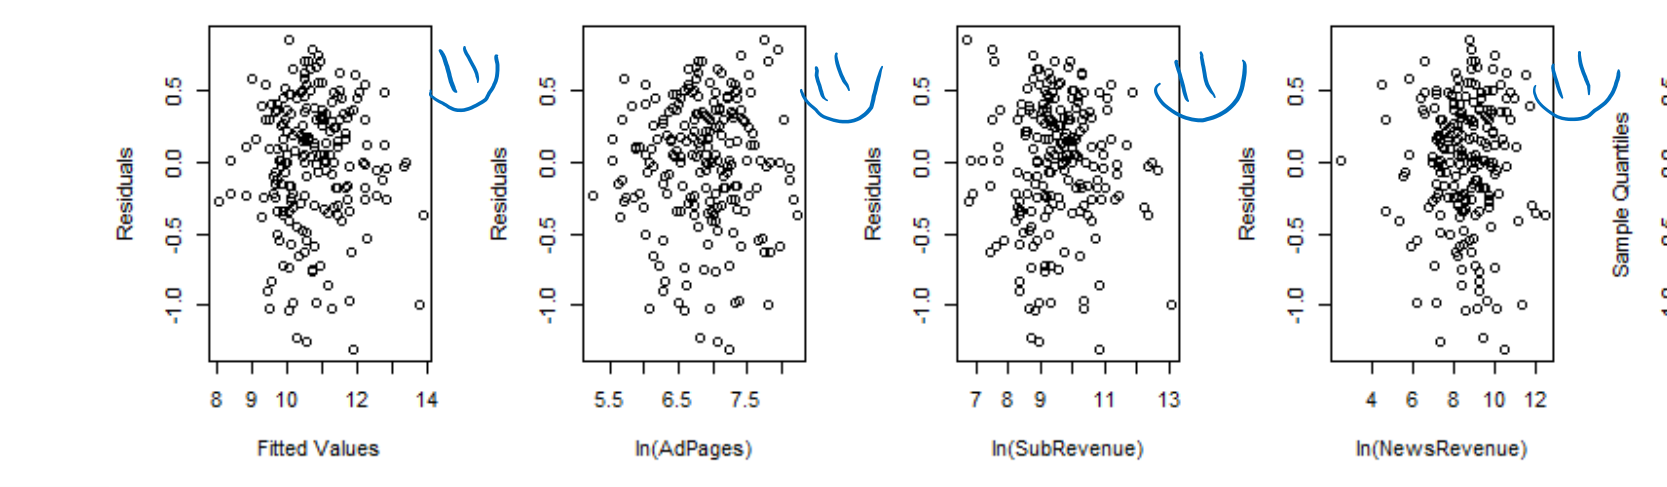
\includegraphics[width=0.85\linewidth]{figures/w4_boxcox_xy_resid.png}
    \end{center}
    \aside{Residual plots look fine; mild C shape in QQ plot.}
\end{example}

\begin{remark}[Interpreting Transformed Models]
    \begin{itemize}
        \item Always interpret using the variables \emph{as they are}: $\log(Y)$, $\log(X)$, etc.
        If a predictor is squared, say ``for a one-unit increase in $x^2$''.
        \item When the response is transformed, predicted values are conditional means
        on the \textbf{transformed scale}, not the original one. We don't
        ``back-transform'' to the original measurement scale.
    \end{itemize}
\end{remark}

\begin{example}[Interpreting the Magazine Model]
    For $\log(Y)\sim\log(X_1)+\log(X_2)+\log(X_3)$:
    \begin{itemize}
        \item \textbf{Intercept}: the expected \textbf{log of Revenue} due to Advertising when
        \textbf{log Ad Pages}, \textbf{log Subscription Revenue} and \textbf{log Newsstand Revenue} are 0.
        \item \textbf{Slope}: for a one unit increase in the \textbf{log of Advertising Pages},
        the slope is the expected change in \textbf{log of Advertising Revenue} for a fixed
        \textbf{log Subscription Revenue} and \textbf{log Newsstand Revenue}.
    \end{itemize}
\end{example}

\subsection{Impact of Violations on Sampling Distributions}

\begin{remark}[Expected Value Vector and Covariance Matrix]
    For a random column vector $\mathbf{Y}=(Y_1,\dots,Y_n)'$:
    $E[\mathbf{Y}]=(E[Y_1],\dots,E[Y_n])'=\boldsymbol\mu$, and
    \[\Var(\mathbf{Y})=\Cov(\mathbf{Y})=E\big[(\mathbf{Y}-E[\mathbf{Y}])(\mathbf{Y}-E[\mathbf{Y}])'\big]\]
    is $n\times n$, with $(i,j)$-th entry $\Cov(Y_i,Y_j)$ and $i$-th diagonal entry $\Var(Y_i)$.
\end{remark}

\begin{proposition}[Linear Transformations]
    Let $\mathbf{Y}$ have mean $\boldsymbol\mu$ and covariance $\boldsymbol\Sigma$, and
    let $\mathbf{A}$ ($n\times p$) and $\mathbf{a}\in\R^p$ be constants. Then
    \begin{center}
        \begin{tabular}{ll}
            $\Var(\mathbf{Y})=E(\mathbf{Y}\mathbf{Y}')-\boldsymbol\mu\boldsymbol\mu'$ & \aside{cf.\ $V(Z)=E(Z^2)-E(Z)^2$} \\
            $E(\mathbf{A}'\mathbf{Y}+\mathbf{a})=\mathbf{A}'\boldsymbol\mu+\mathbf{a}$ & \aside{cf.\ $E(cZ+d)=cE(Z)+d$} \\
            $\Var(\mathbf{A}'\mathbf{Y}+\mathbf{a})=\mathbf{A}'\boldsymbol\Sigma\mathbf{A}$ & \aside{cf.\ $V(cZ+d)=c^2V(Z)$}
        \end{tabular}
    \end{center}
    If $\mathbf{Y}\sim N(\boldsymbol\mu,\boldsymbol\Sigma)$, then
    $\mathbf{A}'\mathbf{Y}\sim N(\mathbf{A}'\boldsymbol\mu,\mathbf{A}'\boldsymbol\Sigma\mathbf{A})$.
\end{proposition}

\begin{remark}[MLR Setup]
    Assuming the assumptions hold, $\mathbf{Y}=\mathbf{X}\boldsymbol\beta+\boldsymbol\epsilon$ with
    $\boldsymbol\epsilon\sim N(\mathbf{0}_n,\sigma^2\mathbf{I}_n)$, i.e.\
    $E[\boldsymbol\epsilon]=\mathbf{0}$, $\Var[\boldsymbol\epsilon]=\mathrm{diag}(\sigma^2,\dots,\sigma^2)$.
    So $\mathbf{Y}$ is multivariate normal too: \hlt{$\mathbf{Y}\mid\mathbf{X}\sim N(\mathbf{X}\boldsymbol\beta,\sigma^2\mathbf{I})$}.
    \\ $\hat{\boldsymbol\beta}=(\mathbf{X}'\mathbf{X})^{-1}\mathbf{X}'\mathbf{Y}$:
    $\mathbf{X}$ is fixed and $\mathbf{Y}$ random, so $\hat{\boldsymbol\beta}$ is random
    (a function of $\mathbf{Y}$); $\boldsymbol\beta$ is an unknown fixed parameter.
    Note $\hat{\boldsymbol\beta}=\mathbf{A}'\mathbf{Y}$ with $\mathbf{A}'=(\mathbf{X}'\mathbf{X})^{-1}\mathbf{X}'$.
\end{remark}

\begin{proposition}[$\hat{\boldsymbol\beta}$ is Unbiased]
    \begin{align*}
        E(\hat{\boldsymbol\beta}\mid\mathbf{X})
        &=E\big((\mathbf{X}'\mathbf{X})^{-1}\mathbf{X}'\mathbf{Y}\mid\mathbf{X}\big)
        =(\mathbf{X}'\mathbf{X})^{-1}\mathbf{X}'E(\mathbf{Y}\mid\mathbf{X})\\
        &=(\mathbf{X}'\mathbf{X})^{-1}(\mathbf{X}'\mathbf{X})\boldsymbol\beta=\boldsymbol\beta
    \end{align*}
\end{proposition}

\begin{proposition}[Variance of $\hat{\boldsymbol\beta}$]
    Using $\Var(\mathbf{A}'\mathbf{Y})=\mathbf{A}'\boldsymbol\Sigma\mathbf{A}$ with
    $\boldsymbol\Sigma=\Var(\mathbf{Y}\mid\mathbf{X})=\sigma^2\mathbf{I}$ and
    $\mathbf{A}=\big((\mathbf{X}'\mathbf{X})^{-1}\mathbf{X}'\big)'=\mathbf{X}(\mathbf{X}'\mathbf{X})^{-1}$
    \aside{($\mathbf{X}'\mathbf{X}$, hence its inverse, is symmetric)}:
    \begin{align*}
        \Var(\hat{\boldsymbol\beta}\mid\mathbf{X})
        &=(\mathbf{X}'\mathbf{X})^{-1}\mathbf{X}'\,\sigma^2\mathbf{I}\,\mathbf{X}(\mathbf{X}'\mathbf{X})^{-1}
        =\sigma^2(\mathbf{X}'\mathbf{X})^{-1}(\mathbf{X}'\mathbf{X})(\mathbf{X}'\mathbf{X})^{-1}
        =\sigma^2(\mathbf{X}'\mathbf{X})^{-1}
    \end{align*}
    \aside{$\sigma^2$ is a scalar, so it can be pulled out front.}
\end{proposition}

\begin{theorem}[Sampling Distribution of $\hat{\boldsymbol\beta}$]
    By linearity of normal random variables,
    \[\boxed{\hat{\boldsymbol\beta}\sim N_{p+1}\big(\boldsymbol\beta,\ \sigma^2(\mathbf{X}'\mathbf{X})^{-1}\big)}\]
    So when the assumptions hold, the estimators are
    \begin{itemize}
        \item \textbf{unbiased} (on average estimate the value they should),
        \item generally \textbf{correlated} (off-diagonals of $(\mathbf{X}'\mathbf{X})^{-1}$ not guaranteed to be 0),
        \item dependent on the same constant variance $\sigma^2$ as the errors.
    \end{itemize}
\end{theorem}

\heading{Violations Break the Sampling Distribution}
\begin{itemize}
    \item \rb{Linearity}: the mean of $\hat{\boldsymbol\beta}$ is no longer $\boldsymbol\beta$ $\Rightarrow$ estimates are biased.
    \item \rb{Constant variance}: no longer a single $\sigma^2$ in the variance.
    \item \rb{Uncorrelated errors}: the variance of the estimators will be under- or over-estimated.
    \item \rb{Normality}: estimators won't have a normal sampling distribution.
\end{itemize}
When assumptions are violated, we don't know the correct way to describe variation
due to sampling $\Rightarrow$ \textbf{inference will be incorrect or misleading}.

\subsection{Gauss--Markov Theorem}

\begin{theorem}[Gauss--Markov (Gauss 1821, Markov 1900)]
    Let $E(\mathbf{Y})=\mathbf{X}\boldsymbol\beta$ \aside{(linearity)}, $\mathbf{X}$ full rank, and
    $\Var(\mathbf{Y})=\sigma^2\mathbf{I}$ \aside{(constant variance, uncorrelated errors)}.
    Then the OLS estimator $\hat{\boldsymbol\beta}=(\mathbf{X}'\mathbf{X})^{-1}\mathbf{X}'\mathbf{Y}$
    is the \textbf{Best Linear Unbiased Estimator (BLUE)} of $\boldsymbol\beta$:
    for any $\mathbf{a}'\boldsymbol\beta$, among estimators that are linear in $\mathbf{Y}$ and
    unbiased, $\mathbf{a}'\hat{\boldsymbol\beta}$ has \textbf{minimum variance}.
    \aside{OLS is the ``best'' --- lowest sampling variance in the class of linear unbiased estimators.}
\end{theorem}

\begin{center}
    \begin{tabular}{p{0.45\linewidth}p{0.45\linewidth}}
        \toprule
        \textbf{Ordinary Least Squares} & \textbf{Maximum Likelihood} \\
        \midrule
        Minimizes \newline $RSS=(\mathbf{Y}-\mathbf{X}\hat{\boldsymbol\beta})'(\mathbf{Y}-\mathbf{X}\hat{\boldsymbol\beta})=\sum_{i=1}^n\hat e_i^2$
        & Maximizes \newline $\ln L(\boldsymbol\beta,\sigma^2\,|\,\mathbf{Y},\mathbf{X})\propto-\frac1{2\sigma^2}\sum_{i=1}^n(y_i-\mathbf{x}_i\boldsymbol\beta)^2$ \aside{(the sum is the RSS)} \\[4pt]
        $\hat{\boldsymbol\beta}=(\mathbf{X}'\mathbf{X})^{-1}\mathbf{X}'\mathbf{Y}$ & $\hat{\boldsymbol\beta}=(\mathbf{X}'\mathbf{X})^{-1}\mathbf{X}'\mathbf{Y}$ \\[4pt]
        Requires: linearity, constant variance, uncorrelated errors. \textbf{No} normality assumption.
        & Requires: linearity, constant variance, uncorrelated errors, \textbf{and normality}. \\
        \bottomrule
    \end{tabular}
\end{center}

\heading{Which Estimation Procedure to Use?}
\begin{itemize}
    \item If normality does not hold, OLS still gives an unbiased and most precise estimator of $\boldsymbol\beta$.
    \item If normality holds, MLE and OLS are equivalent (and both BLUE).
    \item OLS is \textbf{always} more precise than any other estimator linear in $\mathbf{Y}$.
    \item If inference (hypothesis tests, CIs) isn't important, OLS is the better choice
    --- but the point of statistics is to do inference.
\end{itemize}
\aside{Ideally, normality is satisfied so OLS and MLE are the same.}

\subsection{Summary}

\begin{center}
\begin{tikzpicture}[node distance=0.6cm and 0.9cm,
    box/.style={draw,align=center,text width=3.1cm,minimum height=1.3cm,font=\small}]
    \node[box] (build) {Build model $+$ make assumptions (Modules 1--2)};
    \node[box,below=of build] (check) {Check all assumptions with residual plots (Module 3)};
    \node[box,right=of check] (viol) {Strong evidence of violations? (Module 3)};
    \node[box,above right=0.1cm and 0.9cm of viol] (fix) {Correct assumptions (practical considerations) (Module 4)};
    \node[box,below right=0.1cm and 0.9cm of viol] (gm) {Gauss--Markov holds: LS unbiased, min.\ variance (Module 4)};
    \node[box,right=of gm,text width=2.6cm] (inf) {Sampling dist.\ $+$ inference (Module 5)};
    \draw[->] (build) -- (check);
    \draw[->] (check) -- (viol);
    \draw[->] (viol) -- node[above left,font=\small]{Yes} (fix);
    \draw[->] (viol) -- node[below left,font=\small]{No} (gm);
    \draw[->] (gm) -- (inf);
    \draw[->] (fix.west) -- node[above,sloped,font=\small\itshape]{repeat as necessary} (build.east);
\end{tikzpicture}
\end{center}

\heading{Approaches to Transformations}
\begin{itemize}
    \item \rb{Variance stabilizing transformation}
    \begin{itemize}
        \item \textbf{Only} on $Y$; corrects non-constant variance (can improve other
        violations, but can also make them worse).
        \item No obvious choice; common: $\ln(y-c)$, $\sqrt{y-c}$ (variance usually increases with $Y$).
        \item Use judgement from the plots and the funnel direction (e.g.\ $\ln(c-y)$).
    \end{itemize}
    \item \rb{Box--Cox transformation} (on $Y$ and/or $X$)
    \begin{itemize}
        \item Corrects non-normality in $Y$ and/or $X$ (sometimes helps non-linearity).
        \item Estimate $Y^\lambda$ and/or $X^\lambda$ by maximum likelihood.
        \item Guide for simpler transformations: $\hat\lambda=0\to\ln(\cdot)$; $\hat\lambda\neq0\to Y^{\hat\lambda}$ or $X^{\hat\lambda}$.
    \end{itemize}
    \aside{Generally: transform $X$ for linearity issues.}
    \item We \textbf{cannot} correct correlated errors after data collection --- it
    \textbf{must} be addressed at the study design / data collection stage.
\end{itemize}

\heading{Workflow}
\begin{enumerate}
    \item Plot data: scatterplot, scatterplot matrix (pairs plot), histogram, \dots
    \item Plot residuals: all residual plots, QQ plot, \dots
    \item Fix the \textbf{worst} violation first with an appropriate transformation.
    \item Check residual plots again after \emph{every} transformation.
    \item Avoid complex/too many transformations --- keep things interpretable, and
    keep in mind what variables represent.
\end{enumerate}
\aside{Weisberg Ch 8 has a good discussion on transformations.}

\begin{remark}[Module Takeaways]
    \begin{itemize}
        \item Why does a variance stabilizing transformation correct non-constant variance?
        \item What is a Box--Cox transformation trying to achieve?
        \item How do we select and implement transformations to correct model violations?
        \item What does this change in how we interpret model coefficients?
        \item Why is it important to attempt to correct model violations?
        \item Why is the OLS estimator the ``best'' estimator?
    \end{itemize}
    \aside{Next week: inference on coefficients and predicted values. The first hour
    of Module 5 (inference on coefficients) is the last material on the term test.}
\end{remark}
